\documentclass[../../Paper.tex]{subfiles}
  
    
\begin{document}


\begin{table}[!t]
\caption{Outputs of all models trained on all datasets; training and testing accuracies were compared between models to assess model fit.}
\begin{tabular}{ccccllll}
\cline{1-4}
\multicolumn{1}{|l|}{\textit{\textbf{Model Type}}}                                                                     & \multicolumn{1}{l|}{\textit{\textbf{Training Images}}} & \multicolumn{1}{c|}{\textbf{Training Accuracy (\%)}} & \multicolumn{1}{l|}{\textbf{Test Accuracy (\%)}} &           & \multicolumn{1}{c}{} &           &           \\ \cline{1-4}
\multicolumn{1}{|c|}{\multirow{4}{*}{\textit{\begin{tabular}[c]{@{}c@{}} \\CNN \\ \\ Learning rate 0.2\end{tabular}}}} & \multicolumn{1}{c|}{Dataset 1}                         & \multicolumn{1}{c|}{99.1}                            & \multicolumn{1}{c|}{31}                          &           &                      &           &           \\ \cline{2-4}
\multicolumn{1}{|c|}{}                                                                                                 & \multicolumn{1}{c|}{Dataset 2}                         & \multicolumn{1}{c|}{99}                              & \multicolumn{1}{c|}{48}                          & \textbf{} & \textbf{}            &           &           \\ \cline{2-4}
\multicolumn{1}{|c|}{}                                                                                                 & \multicolumn{1}{c|}{Dataset 3-NORM}                    & \multicolumn{1}{c|}{92.2}                            & \multicolumn{1}{c|}{55}                          &           &                      &           &           \\ \cline{2-4}
\multicolumn{1}{|c|}{}                                                                                                 & \multicolumn{1}{c|}{Dataset 3}                         & \multicolumn{1}{c|}{93.9}                            & \multicolumn{1}{c|}{57}                          &           &                      &           &           \\ \cline{2-4}
\multicolumn{1}{|c|}{}                                                                                                 & \multicolumn{1}{c|}{Dataset 4}                         & \multicolumn{1}{c|}{98.6}                            & \multicolumn{1}{c|}{94}                          &           &                      &           &           \\ \cline{1-4}
\multicolumn{1}{|c|}{\textit{\begin{tabular}[c]{@{}c@{}}CNN \\ Learning rate 0.15\end{tabular}}}                    & \multicolumn{1}{c|}{Dataset 3}                         & \multicolumn{1}{c|}{88.3}                            & \multicolumn{1}{c|}{62}                          &           &                      &           &           \\ \cline{1-4}
\multicolumn{1}{|c|}{\multirow{5}{*}{\textit{\begin{tabular}[c]{@{}c@{}}Random Forest\\ 100 trees\end{tabular}}}}      & \multicolumn{1}{c|}{Dataset 1}                         & \multicolumn{1}{c|}{99.8}                            & \multicolumn{1}{c|}{42}                          &           &                      &           &           \\ \cline{2-4}
\multicolumn{1}{|c|}{}                                                                                                 & \multicolumn{1}{c|}{Dataset 2}                         & \multicolumn{1}{c|}{99.4}                            & \multicolumn{1}{c|}{45}                          & \textbf{} &                      & \textbf{} & \textbf{} \\ \cline{2-4}
\multicolumn{1}{|c|}{}                                                                                                 & \multicolumn{1}{c|}{Dataset 3-NORM}                    & \multicolumn{1}{c|}{95.9}                            & \multicolumn{1}{c|}{57}                          &           &                      &           &           \\ \cline{2-4}
\multicolumn{1}{|c|}{}                                                                                                 & \multicolumn{1}{c|}{Dataset 3}                         & \multicolumn{1}{c|}{96}                              & \multicolumn{1}{c|}{62}                          & \textbf{} & \textbf{}            & \textbf{} & \textbf{} \\ \cline{2-4}
\multicolumn{1}{|c|}{}                                                                                                 & \multicolumn{1}{c|}{Dataset 4}                         & \multicolumn{1}{c|}{97.9}                            & \multicolumn{1}{c|}{94}                          &           &                      &           &           \\ \cline{1-4}
\multicolumn{1}{|c|}{\multirow{2}{*}{\textit{\begin{tabular}[c]{@{}c@{}}Random Forest\\  500 trees\end{tabular}}}}   & \multicolumn{1}{c|}{Dataset 2}                         & \multicolumn{1}{c|}{99.4}                            & \multicolumn{1}{c|}{48}                          &           &                      &           &           \\ \cline{2-4}
\multicolumn{1}{|c|}{}                                                                                                 & \multicolumn{1}{c|}{Dataset 3}                         & \multicolumn{1}{c|}{96.3}                            & \multicolumn{1}{c|}{60}                          &           &                      &           &           \\ \cline{1-4}

\end{tabular}
\end{table}

All model results were noted, and models were adjusted as we saw fit; the number of trees in the Random Forest model were adjusted, as were the CNN models learning rates (Table 2). These were changed to assess the impacts on the model accuracies. 

All CNN models were stopped between 3000 and 5000 training iterations; accuracies had exceeded 90\% by this time, and model loss (the number of inaccurate predictions) was \textless 0.20 (Figure 5). Allowing the model to run for excess iterations did not improve the training accuracy nor did it drastically improve the loss; stopping the models allowed for over-fitting to be minimised whilst also allowing model losses to remain low.



\begin{figure}[!b]
\begin{subfigure}{.5\textwidth}  
\centering
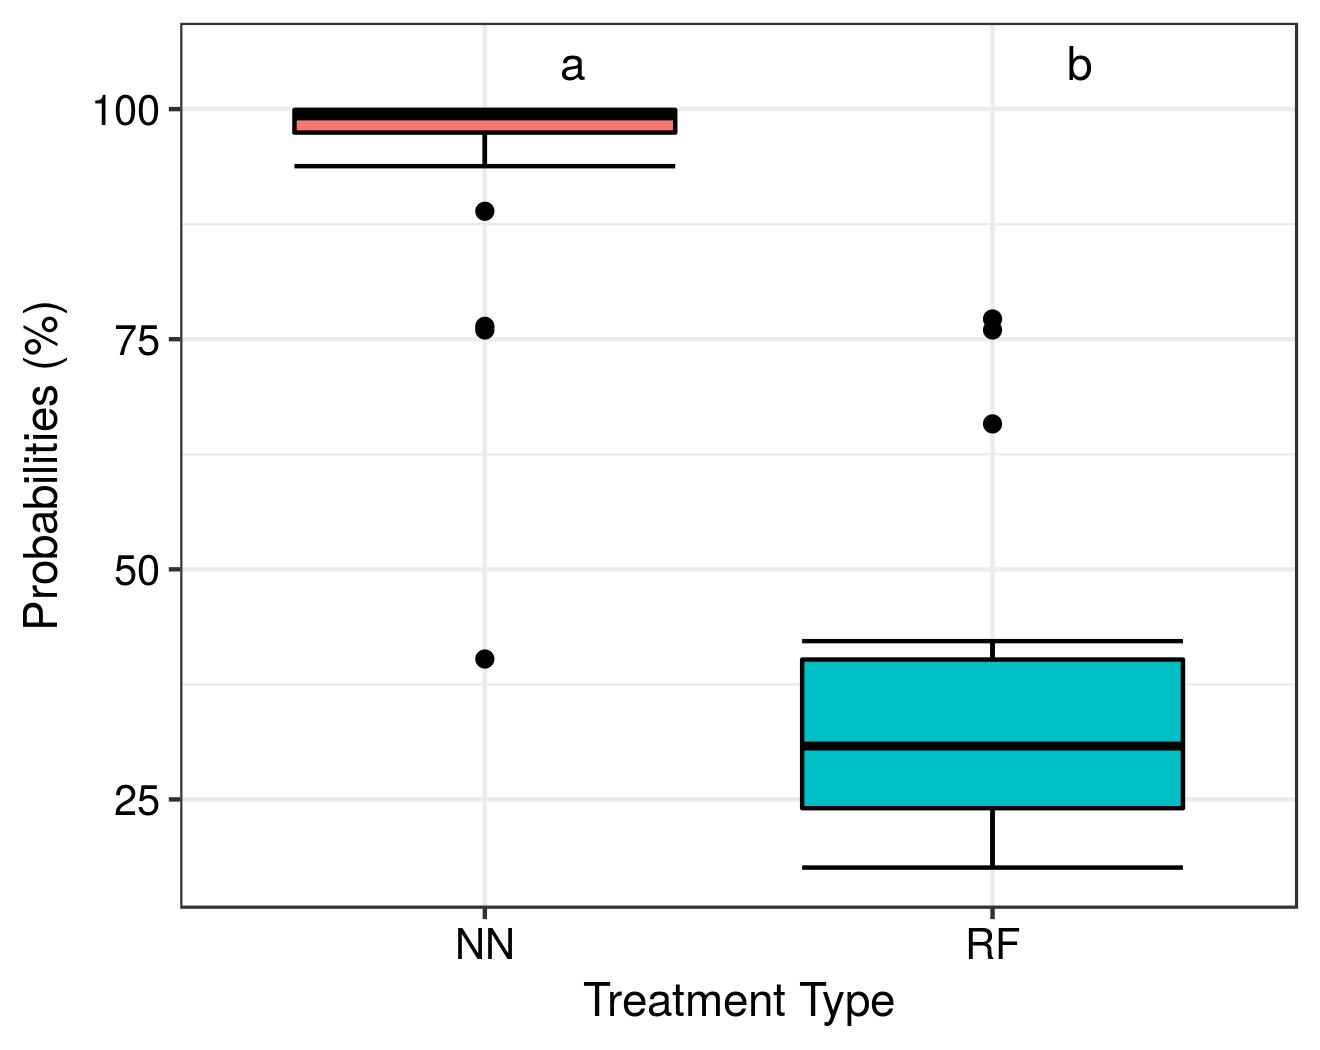
\includegraphics[scale = 0.6]{CNN_treatment.jpg}
\caption{Results for treatment models trained on dataset 3. CNNs were significantly more certain (p \textless 0.0001) in comparison to RFs.}
  \label{fig:sub2}
\end{subfigure}
\begin{subfigure}{.5\textwidth}
  \centering
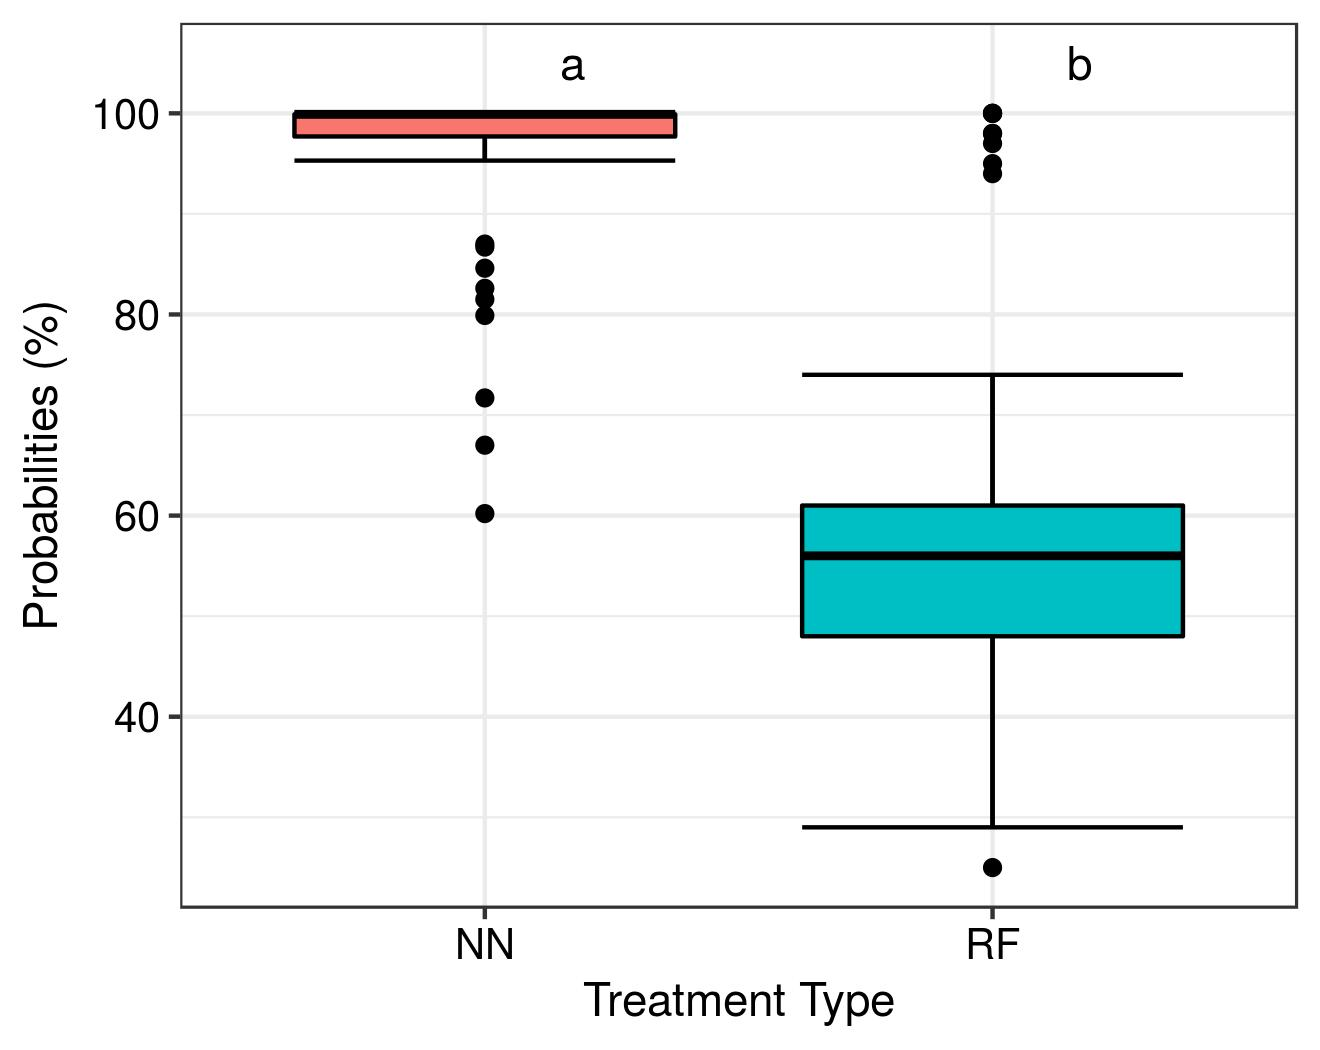
\includegraphics[scale = 0.6]{CNN_duration.jpg}
\caption{Results for duration models trained on dataset 4. CNNs were significantly more certain (p \textless 0.0001) in comparison to RFs.}
  \label{fig:sub1}
\end{subfigure}
\caption{True Positive test accuracy results for RF and CNN models trained on multi-stress dataset 3 and duration dataset 4. }
\label{fig:test}
\end{figure}

\subsection*{Multi-stress treatments}

Results from the multi-stress classification show both algorithms correctly classify all  datasets (1-3), with accuracy increasing with additional colour-pass filters. However, accuracy decreased when using the normalised dataset (3-NORM).


Both RFs and CNNs returned high ( \textgreater  88\% ) training accuracies for all datasets; training accuracies decreased as datasets contained more colour-pass filter images (Table 2). Despite this, testing/ validation accuracies increased as more colour-pass images were included. Models trained on the normalised dataset (Dataset 3-NORM) returned lower accuracies in comparison to Dataset 3 (Table 2).


Due to both CNN and RF models returning similar accuracy ratings, the percentage certainties of correct predictions were compared (Figure 6a). The outcome of this comparison was that the CNN models predictions were significantly more certain than that of the RFs (ANOVA: $F_{1,50}$ = 218.1 , p \textless 0.0001). 



\subsection*{Duration Infection}

Results from the duration infection classification show both algorithms can correctly classify dataset 4.

Both RF and CNNs managed to return a \textgreater 97\% training accuracy and a 94\% testing accuracy (Table 1); when true positive prediction certainties were compared (Figure 6b), CNNs were found to be significantly more certain in comparison to the RF model (ANOVA: $F_{1,120}$ = 216.3, p \textless 0.0001). 


\subsection*{Pixel Intensities}

Pixel intensities for both multi-stress and infection duration treatments show that all treatments are statistically different from one another, allowing for further support of the models classification results.


\begin{figure}[!b]
  \centering
  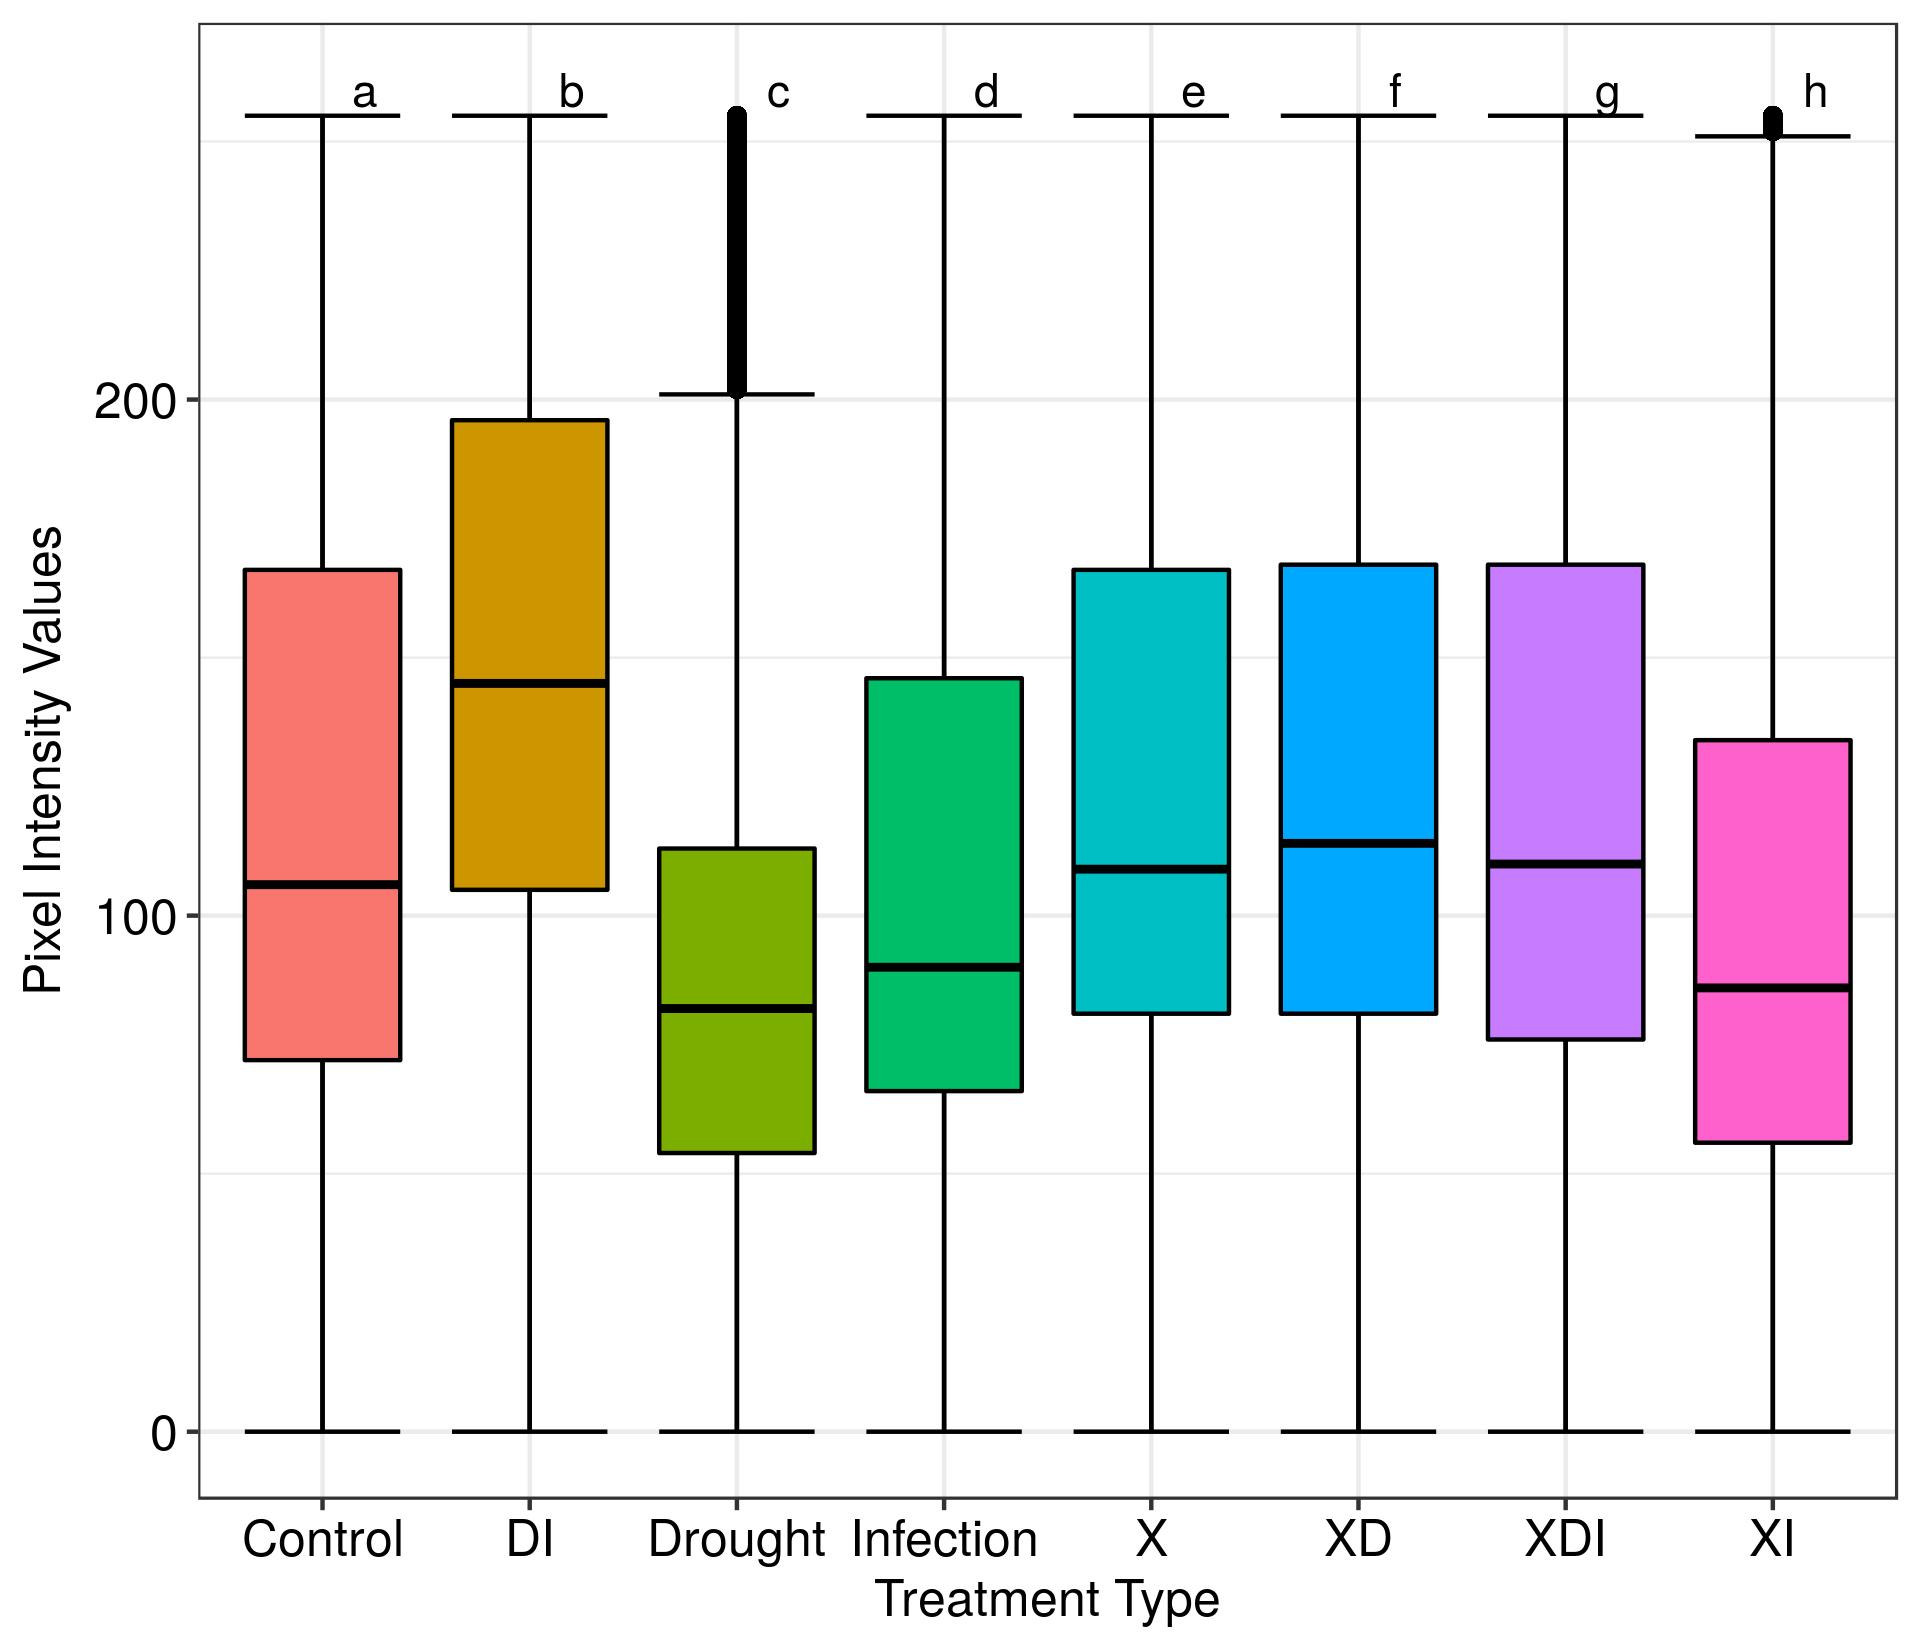
\includegraphics[scale = 0.67]{treatments3.jpg}
  \caption{Pixel Intensities of the multi-stress dataset (RGB images only). All treatments were proven to be statistically different from one another.}
  \label{fig:sub1}
\end{figure}

\begin{figure}[!t]
  \centering
  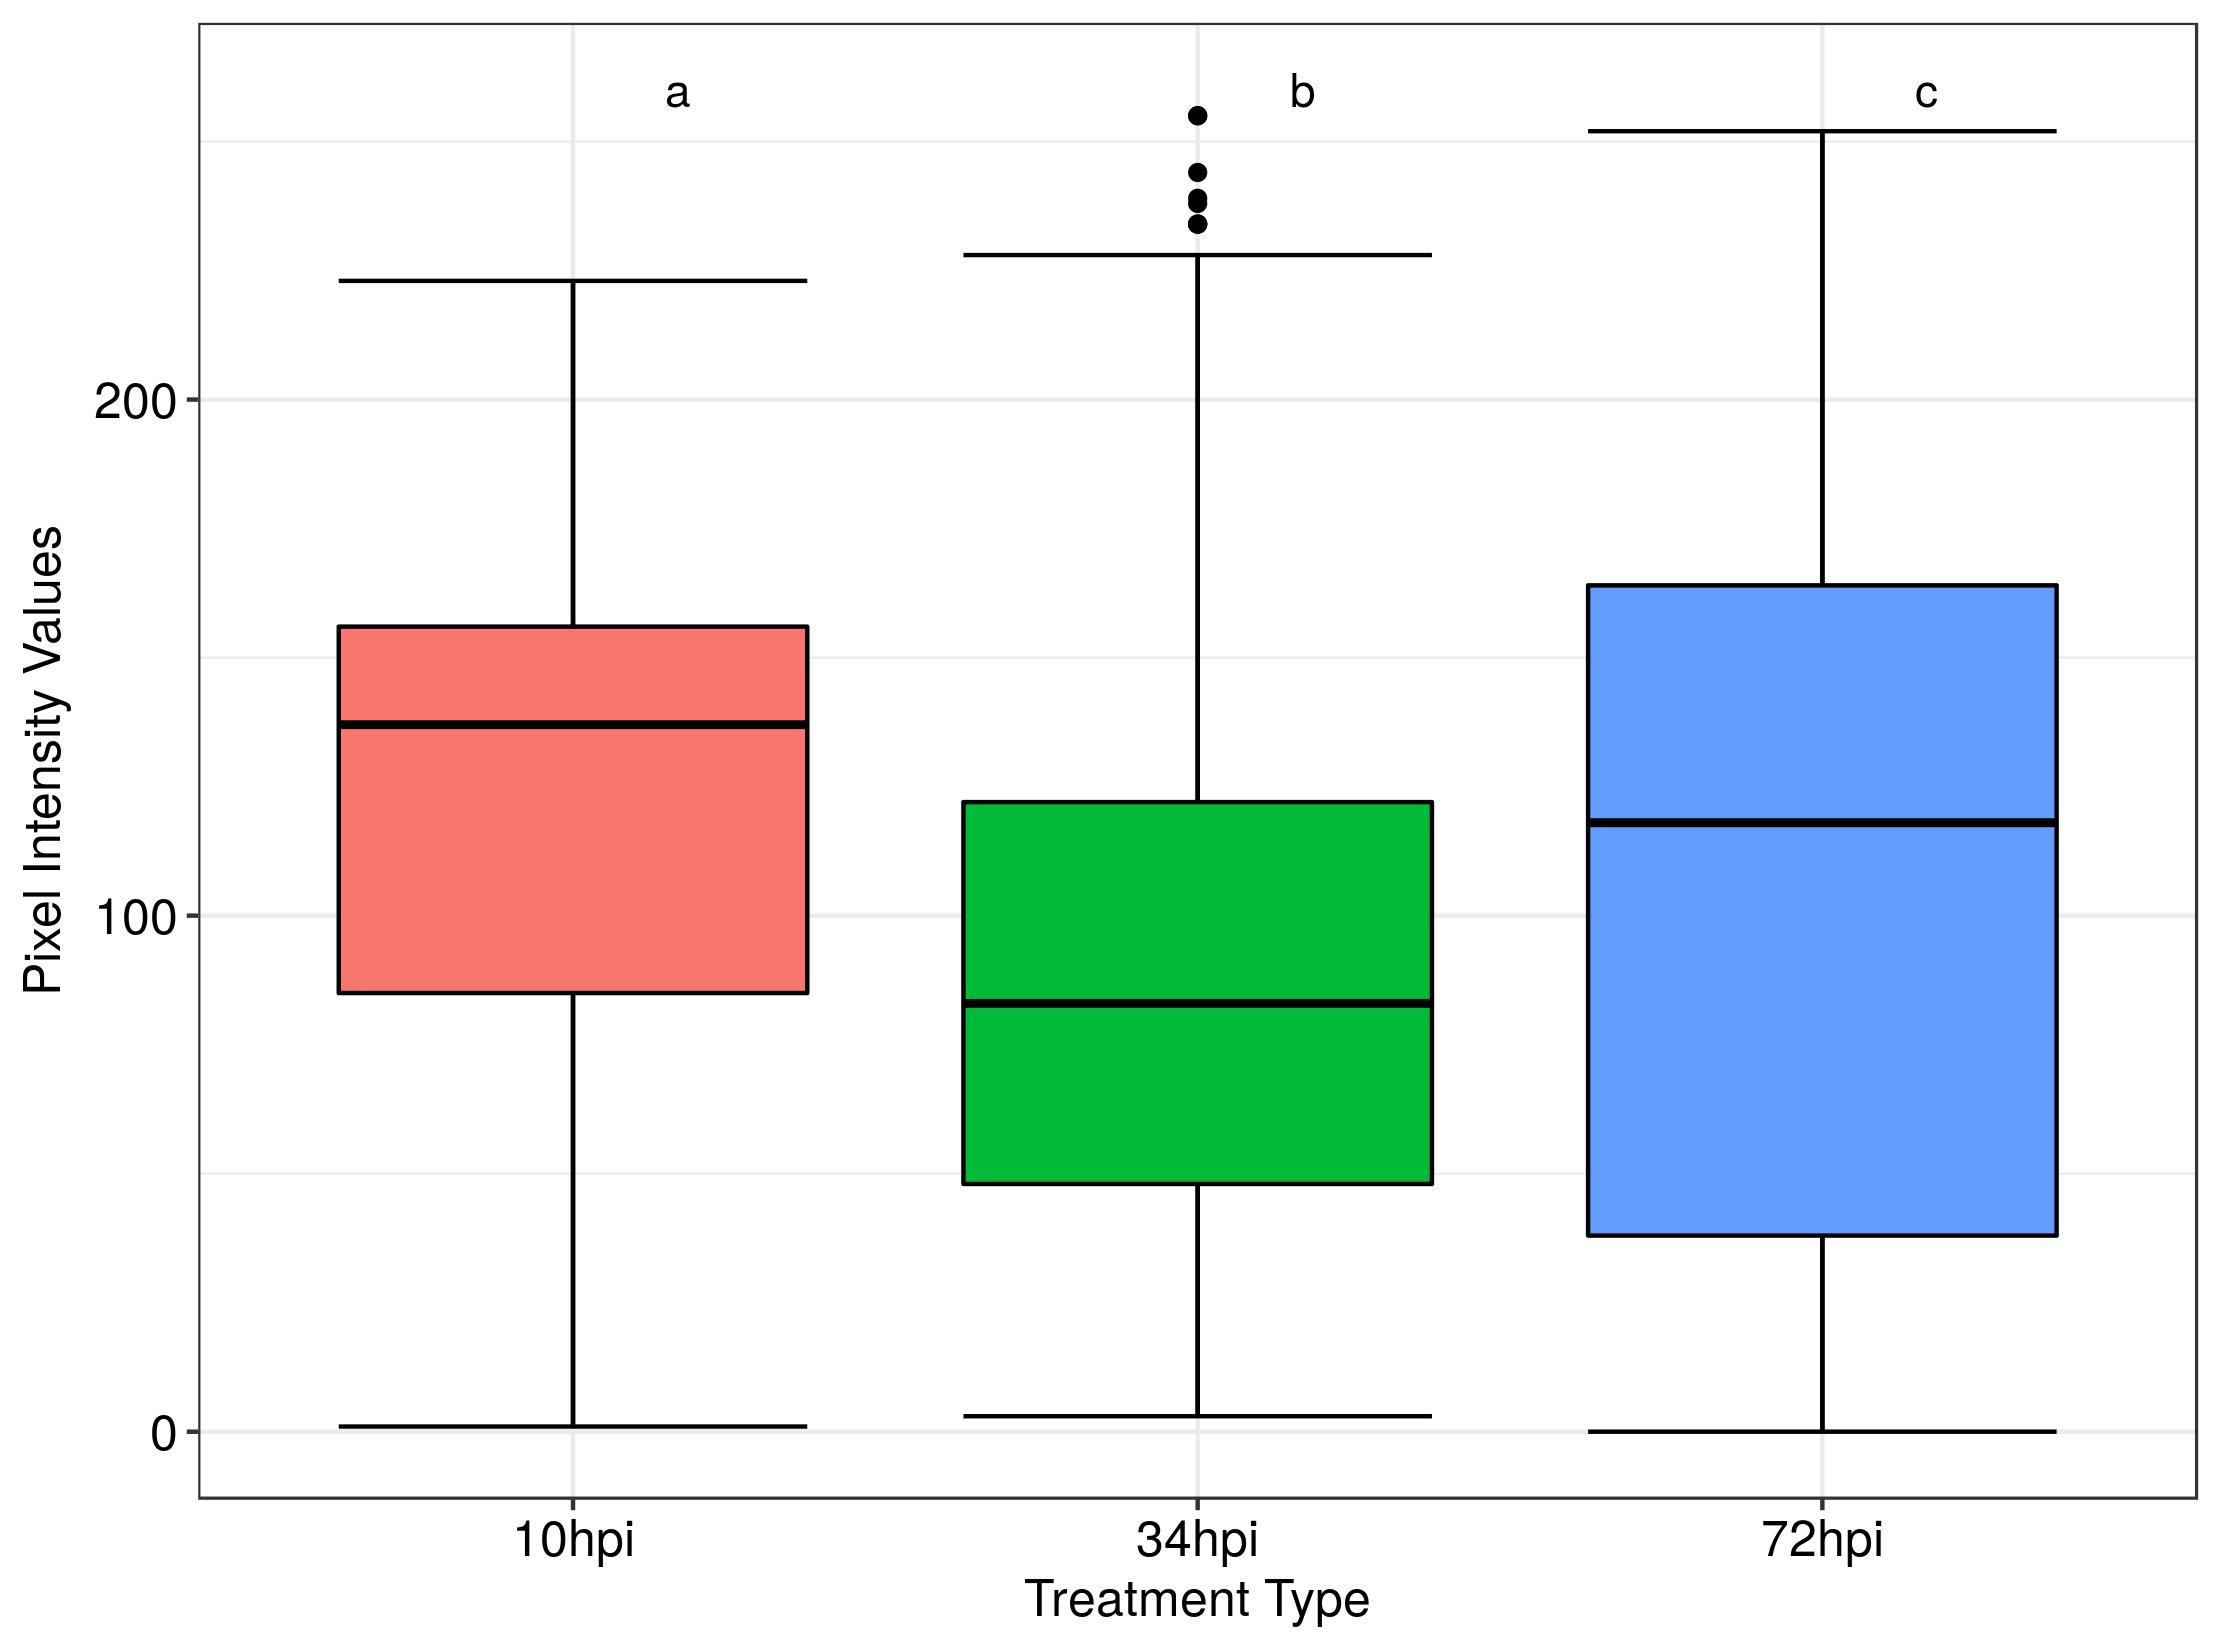
\includegraphics[scale = 0.60]{treatments11.jpg}
  \caption{Pixel Intensities for part of the infection duration dataset (dataset 4). All treatments were proven to be statistically different from one another.}
  \label{fig:sub2}
\end{figure}

When pixel intensities were compared between treatments, both multi-stress and duration infection treatments returned significant results (ANOVA multi-stress:  $F_{7,4646161}$ = 38676, p \textless 0.0001; ANOVA duration infection:  $F_{2,1628925}$ = 32894,  p \textless 0.0001); Figures 7 and 8 show that all treatment types were significantly different from one another. Further comparison shows that channels significantly differ both within and between treatments (ANOVA duration infection: Appendix Figure 1, $F_{8,1628919}$ = 3437540,  p \textless 0.0001; ANOVA multi-stress: Appendix Figure 2, $F_{23,4646145}$ = 17195, p \textless 0.0001)


\end{document}